\part[Analysis of the Folding of Myotrophin with a Simple Model]
{Analysis of the Folding of Myotrophin with the Wako-Saito-Mu{\~n}oz-Eaton Model
%WSME - protein equilibrium and kinetics
}

\sectionnonum{Introduction}
\thispagestyle{plain}

\lettrine{I}{n} this part of this Thesis we will 
apply the Wako-Saito-Mu{\~n}oz-Eaton (WSME) model to the study
of Myotrophin, a small ankyrin repeat protein, whose folding 
equilibrium and kinetics  have been recently characterized experimentally. 

Modular proteins are frequently found in proteome databases, and they are
identified mainly in eukaryotes proteomes, but are abundant also in prokaryotes. The natural abundance of proteins
containing duplicated sequence reach 14\% \cite{marcotte1999}, 
which double if we restrict only to eukaryote proteins.
In particular the ankyrin motif represents one of the most frequently observed motifs 
in repeat protein structures, which is composed by two anti-parallel helices
followed by a $\beta$-hairpin or a long loop (see figure \ref{fig:prot}).
In particular in rats, Myotrophin is found to be related to the heart muscle
hypertrophy in which this protein over-express.

Modular proteins drawn researchers interests, providing a different folding
paradigm with respect to the well known
one of globular proteins, where complex native state geometries, 
characterized by local and non-local interactions, are most often associated 
to a simple two-state equilibrium and kinetics.
On the contrary, repeat proteins are characterized by tandem arrays 
of the same structural motif (even if individual repeats show just 
partial sequence identity, typically, around 25\% \cite{Kloss2008}). 
Such motifs are usually arranged in a linear fashion, giving rise to elongated 
structures that may consist of a highly variable number of repeats. 
Due to this characteristic this kind of proteins are more likely to lack  an
active site and generally act in the cell processes as building blocks
(connective tissue proteins, cytoskeletal proteins\dots) \cite{marcotte1999} or
 as a scaffold for various protein-protein interaction \cite{Mosavi2004}.

Interactions in such modular structures take place within a repeat 
and between adjacent repeats, while truly non-local interactions connecting 
non-contiguous repeats are lacking. While such organization provide a 
general-purpose scaffold that can be tuned to bind different species, 
it is quite surprising that it is still compatible with a cooperative, 
two-state folding. 
Indeed, recent experimental studies have revealed that repeat proteins 
typically show a two-state equilibrium but a multi-state kinetics \cite{Kloss2008}, 
driving the attention on the existence of different folding pathways. 
From a theoretical point of view, repeat proteins provide an ideal 
framework for modelling and hypothesis-testing, due to their structural 
modularity, and to the fact that artificial molecules can be built 
from consensus sequences, so that the role of the different interactions 
and of the chain length can be dissected and analysed individually.

Not surprisingly, the classical  Ising model from statistical mechanics 
has been used to  describe these almost linear systems with local 
nearest-neighbour interactions, where the spin variables have been 
identified with individual helices within a repeat \cite{Kaj2005}, 
or with entire repeats \cite{Wetzel2008}, or with the elementary 
\emph{foldons} identified in a more detailed molecular dynamics simulation 
\cite{Ferreiro2008}. Typically, the external fields and neighbour 
interaction parameters ($h_i$ and $J_{i,i+1}$ respectively, in their 
typical textbook denominations) are derived from the experimental analysis 
of the stability of constructs
of different length, and are related to the variation of the areas accessible 
to the solvent in the folding process.

The identification of the elementary spin variable with a piece of structure 
as a whole, hinders the possibility to investigate the detailed 
role of individual contacts between the residues, and of studying the origin 
of the cooperativity and multi-state kinetics on the residue scale. 

Here, we use the Wako-Saito-Mu{\~n}oz-Eaton (WSME) model 
\cite{Wako1978a,Wako1978b,Munoz1998,Munoz1997,Munoz1999}, 
where the state of each residue $i$ is described by a binary variable 
$m_i=0,1$, representing the unfolded and native state, respectively. 
Formally, the model differs from the Ising one in that the interactions 
are not limited to next neighbours, but extend to any distance, provided 
that the variables corresponding to all the intervening residues are set 
to the native state. The model equilibrium can be exactly calculated 
\cite{Wako1978a,Wako1978b,Bruscolini2002,Pelizzola2005}, so that energies, 
free-energies, and fractions of native residues can be easily evaluated.
The folding and unfolding kinetics are studied through Monte Carlo simulation, 
with an elementary step corresponding to the folding/unfolding of one residue. 

The model has been applied to describe the folding of many proteins 
\cite{Zamparo2009,Cellmer2008,Itoh2008,Itoh2010,Abe2009,Morozov2007,
Chung2008,Bruscolini2007a,Bruscolini2007},
and also to the study of force-induced denaturation of proteins and RNA 
\cite{Imparato2007,Imparato2007a,Imparato2008,Imparato2009,Caraglio2010}. 
We apply the WSME model to the study of Myotrophin, a 118 residues protein, 
ubiquitously expressed in all mammalian tissues 
\cite{Sen1990,Taoka1994,Sivasubramanian1996,Anderson1999}, 
made up of four ankyrin repeats. 
This molecule, a cardiomyogenic hormone,  is found to be over-expressed in
hypertrophied heart muscle \cite{Mukherjee1993}.
Its equilibrium has been characterized 
experimentally as two-state  by Peng and co-workers\cite{Mosavi2002a}
with thermal and chemical denaturation experiments, and later confirmed 
as such, at least as far as chemical denaturations is concerned, 
by  Lowe and Itzhaki \cite{Lowe2007a}, that also studied the kinetics 
\cite{Lowe2007a,Lowe2007}. 
In the former paper, the authors propose an effective two-state framework 
to interpret the relaxation kinetics \cite{Lowe2007a} 
(more precisely, they actually observe some curvature in the unfolding arm 
of the chevron plot, that can be explained by postulating either a barrier 
shift or the existence of a high energy intermediate of negligible population).
\begin{figure}
\centering
\subfigure{
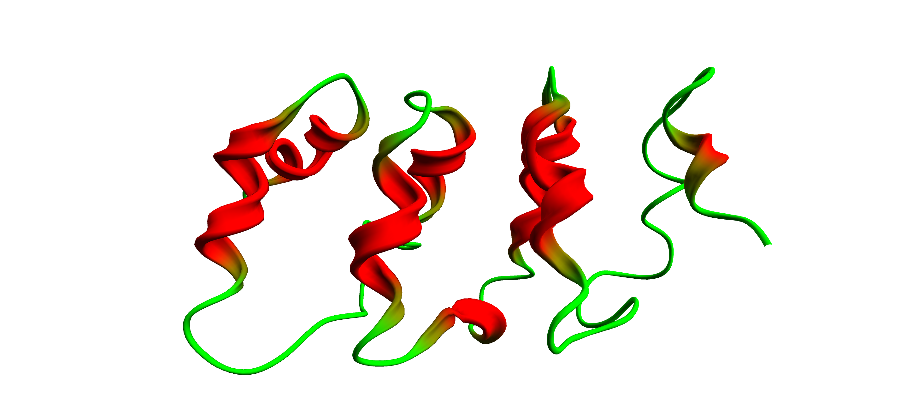
\includegraphics[width=0.8\textwidth]{./img/wsme/2MYO-g.eps}}
\subfigure{
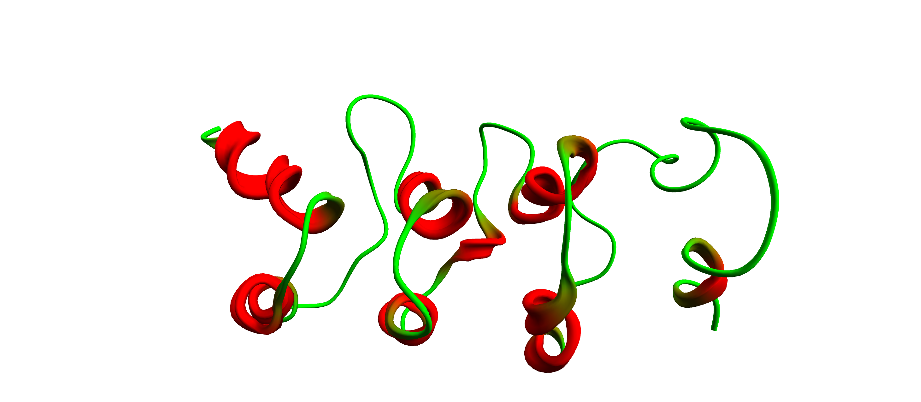
\includegraphics[width=0.8\textwidth]{./img/wsme/2MYO-v-g.eps}}
%\caption{
\begin{minipage}{0.9\textwidth}
\flushleft
\small
\refstepcounter{partintro}
{\bf Figure \arabic{partintro}:}
\label{fig:prot}Sketched view of Myotrophin from the side
\emph{(top)} and from the top \emph{(bottom)}. The molecule is composed of 118
residue which secondary structure is composed of seven $\alpha$-helices and one
$\pi$-helix, ordered in four pairs. Each pair of helices represents an ankyrin
repeat. The picture is based on the structure characterized by
\cite{Yang1998} and published on the Protein Data Bank as 2MYO.
\end{minipage}
%}
\end{figure}

An extended analysis on several mutants leads them to conclude that, 
in order to explain within a unique framework the behaviour of both the 
wild type and the mutants, pathway heterogeneity must be assumed, 
with the dominant pathway presenting a high energy intermediate, 
which is lacking in the secondary one \cite{Lowe2007}. 

Even if their analysis contains several simplifying assumptions 
(for instance, the fact that the relaxation rate is just the sum of the rates 
along the two pathways) they are able to provide very good fits to 
the experimental data, and to determine that the two pathways present 
different nucleation sites, on the N-terminal or on the C-terminal part 
of the protein, respectively. Finally, they show how, by combining mutations, 
it is possible to make the protein switch between the two pathways.

After fitting the model parameters  to reproduce the fraction of native 
protein as a function of the denaturant concentration derived from experiments, 
we calculate  the free energy profiles and relaxation rates, and characterize 
the relaxation pathways, at low and high denaturant concentrations, for the wild 
type protein and for a series of mutants, selected to probe different regions 
and contact distances. We also simulate the set of mutations used in 
Ref.~\cite{Lowe2007}, to test the double pathway hypothesis.

Our goal is to  reproduce, at least qualitatively, the experimental behaviour, 
and to shed light on the nature of the folding nuclei, as well as to recover 
the role of ``pathway switch'' played by some mutations. 
Moreover, we want to clarify the different role played by mutations affecting 
local or non-local contacts in the same region.


%\begin{figure}
%\centering
%\includegraphics[width=0.4\textwidth,angle=-90]{./img/wsme/seq-alignment-2myo.eps}
%\caption{Sequence alignment of Myotrophin. Alignment of identical residue
%strings with length higher or equal to two residues is reported (dark areas means that
%residue $i$ and residue $j$ belong to helices). It is clear that the repeated
%strings does not represent an important part of the repeating modules.
%{\bf??? non so se mettere questo grafico???}}
%\end{figure}

According to the above considerations, the outline of this part is as follows:

\paragraph{WSME model}

In chapter \ref{chap:wsme-model} we review the model introducing a small
modification to deal chemical as well thermal denaturation.
The system parameters are fitted to agree with the experimental Myotrophin equilibrium denaturation
curves in order to test the model against the published data.
We introduce and discuss several relevant observables to explain the equilibrium
and kinetics results, as well the strategy we use to mimic mutation and to
identify the pathway heterogeneity proposed by \citet{Lowe2007}.
Thanks to the model characteristics we have a fine control over the folding
processes and we can ideally follow each molecule step by step. 


\paragraph{Application and Results}

In chapter \ref{chap:wsme-results} we present the results of application of the WSME model
to the protein Myotrophin, including comparison with experimental
studies for the equilibrium and kinetics data.

We show that the overall two-state-like equilibrium and kinetics of the wild
type protein can hide a non-trivial free-energy profile. 
These features appear to be related to a careful 
``design'' of the free-energy landscape where the intermediates are always at
high energy, so that mutations can alter this picture, 
stabilizing some intermediates and changing the position of the rate-limiting step. 

Furthermore the heterogeneity of folding pathways is qualitatively reproduced as
the model predicts two distinct folding  pathways, one through the N-terminal and the other through the 
C-terminal part, even if the variations in the rates 
upon the experimental mutations cannot be quantitatively reproduced. 
Interestingly, folding and unfolding pathways appear to be different, 
even if closely related: a property that is not generally considered 
in the phenomenological interpretation of the experimental data.
